\section{Evaluation}
\label{sec:eval}

We evaluated our solver for a class table containing more than 40000 classes exported by the symbolic execution engine using
nine benchmark queries of various shapes. The results are presented in Fig.~\ref{fig:eval-diagram} in the form of
a bar chart. Here the groups of four bars correspond to different benchmarks, each bar in the group corresponds to a one of
four versions of the solver (left-to-right): with no optimizations, with dynamic transitive closure only, with dynamic class table specialization only,
and with both optimizations enabled.

The benchmark queries are as follows:

\begin{enumerate}
   \item $\alpha$ $\precprec$ \java{java.util.List<Object>}
   \item $\alpha$ $\precprec$ \java{java.util.RandomAccess} $\land$ \\
          $\alpha$ $\precprec$ \java{java.util.AbstractCollection<Object>}
    \item $\alpha$ $\precprec$ \java{java.util.AbstractCollection<Object>} $\land$ \\
          $\alpha$ $\precprec$ \java{java.util.RandomAccess} 
    \item $\alpha$ $\precprec$ \java{java.util.AbstractCollection<Object>} $\land$ \\
          $\alpha$ $\precprec$ \java{java.util.RandomAccess} $\land$ \\
          $\alpha$ $\precprec$ \java{java.util.List<Object>}
    \item \java{javax.management.AttributeList} $\precprec$ $\alpha$
    \item \java{javax.management.AttributeList} $\precprec$ $\alpha$ $\land$ \\
          \java{kotlinx.collections.PersistentVector<Object>} $\precprec$ $\alpha$
    \item \java{kotlinx.collections.PersistentVector<Object>} $\precprec$ $\alpha$ $\land$ \\
          \java{javax.management.AttributeList} $\precprec$ $\alpha$ $\land$ \\
          \java{com.google.common.collect.ImmutableSortedSet<Object>} $\precprec$ $\alpha$
    \item \java{kotlinx.collections.PersistentVector<Object>} $\precprec$ $\alpha$ $\land$ \\
          $\alpha$ $\precprec$ \java{java.util.List<Object>}
    \item $\alpha$ $\precprec$ \java{java.util.List<Object>} $\land$ \\
          \java{kotlinx.collections.PersistentVector<Object>} $\precprec$ $\alpha$
\end{enumerate}


%\begin{itemize}
%    \item The first founr queries are systems of one, two, and three inequations with upper bounds only 1, 2 and 3 upper bounds for standard collection classes and interfaces \java{List}, \java{Abstract%Collection} and \java{RandomAccess}. Note, the 2nd and the 3rd queries are the same 2 upper bounds but with opposite order.
%    \item The next 3 queries are 1, 2 and 3 lower bound for concrete collection classes \java{AttributeList}, \java{PersistentVector} and \java{ImmutableSortedSet}.
%    \item The last 2 queries consist of one upper bound and one lower bound. These bounds the same for both queries but with opposite order.
%\end{itemize}

\begin{figure}[t]
  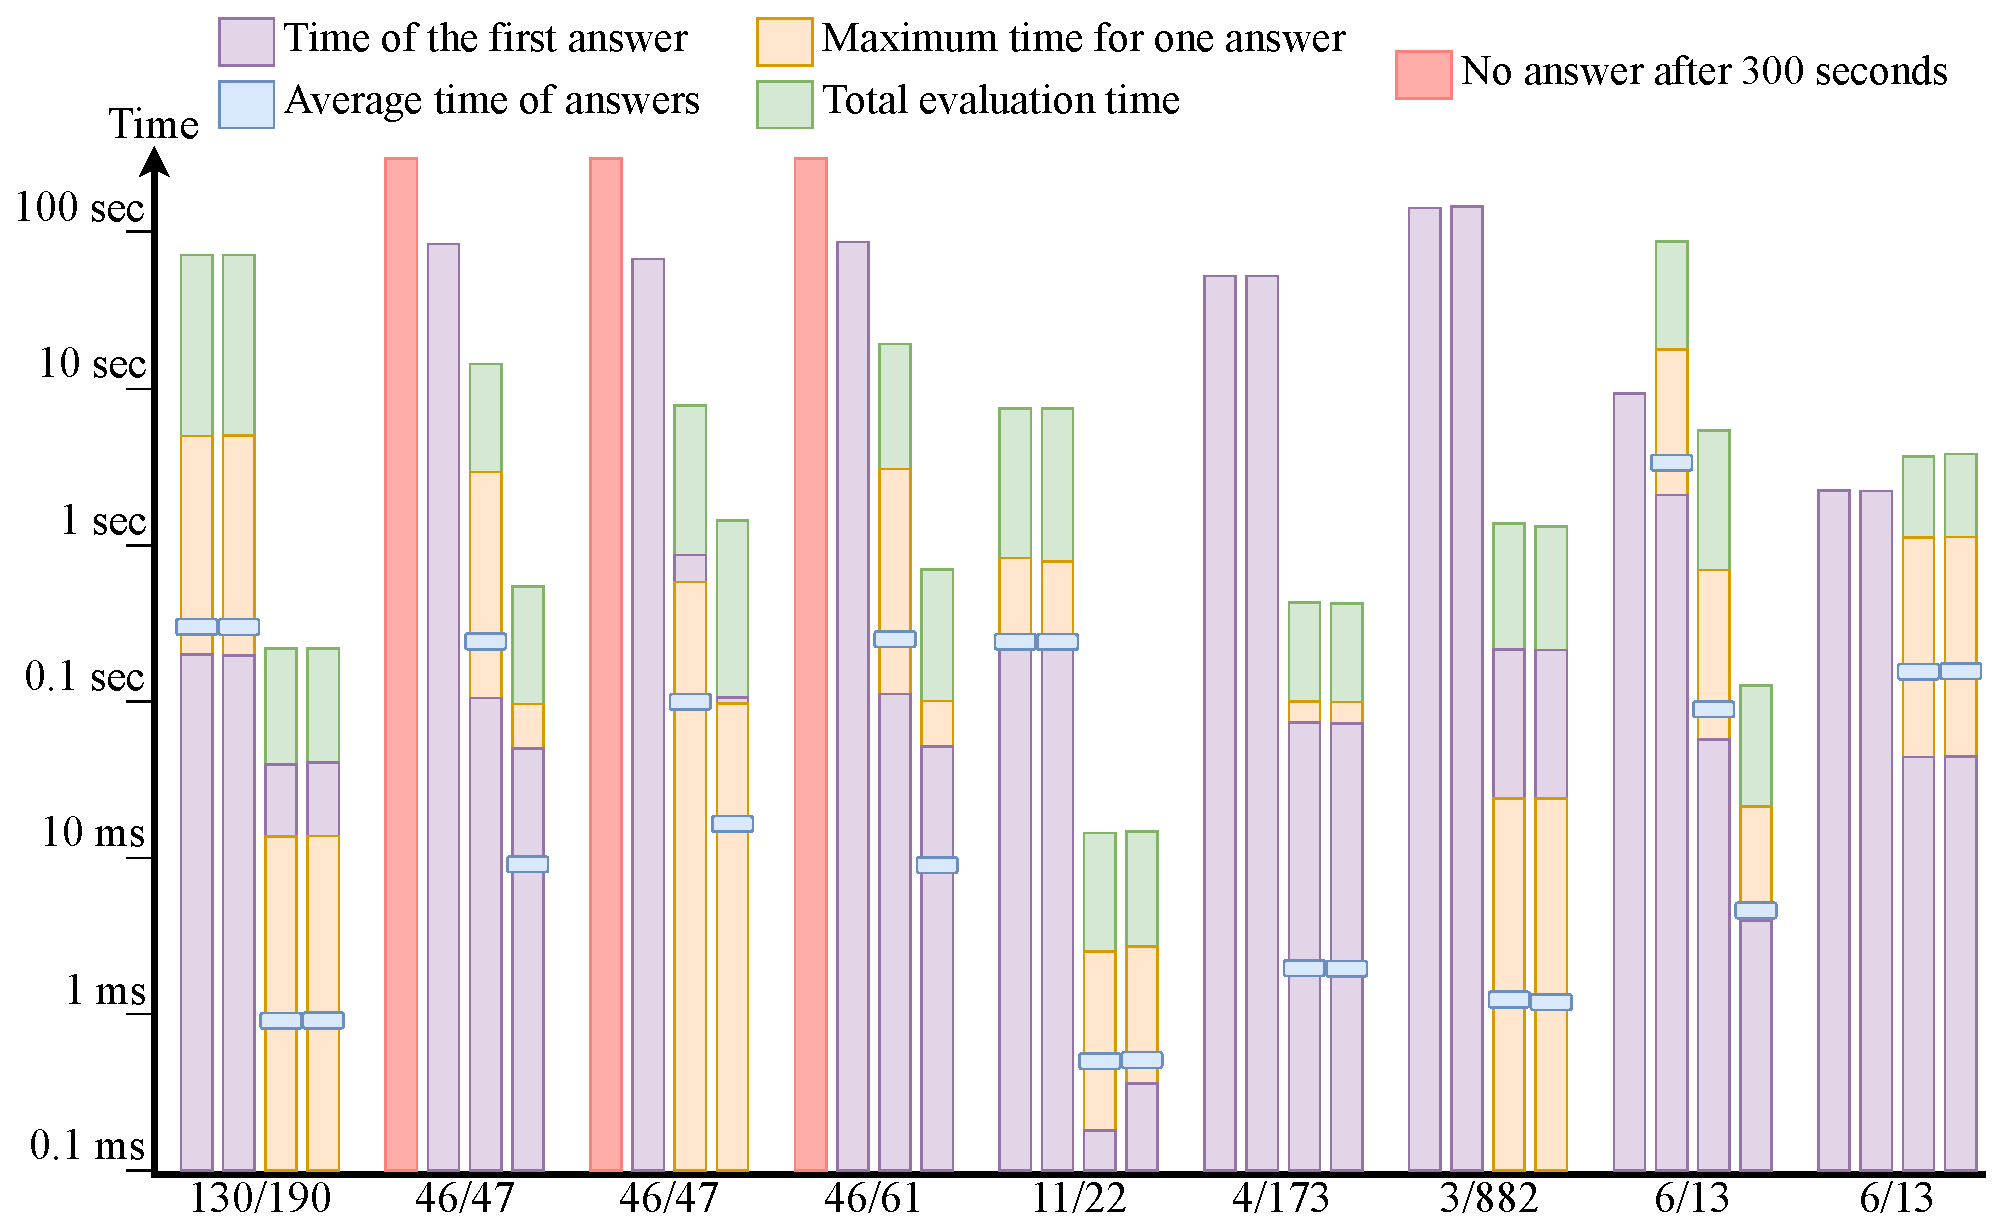
\includegraphics[width=1\textwidth]{eval_diagram.eps}
  \caption{Evaluation results}
  \label{fig:eval-diagram}
\end{figure}

 For each query we evaluated two quantitative measures: the overall number of aswers (shown as a numerator
under corresonding benchmark) and the number of unique answers (shown as a denominator). Also we evaluated four time measures: the time of calculating the first answer (this time includes the time
spent on the pre-calculations required by dynamic table specialization), the maximal time for one answer (not including the first answer time), the average time taken over all answers,
and the total evaluation time. We also limited the evaluation time to 300 seconds; in a few cases we either received only a part of the answers (in this case, only the time for
calculating the first answer is indicated), or we did not receive a single answer (in this case, the red column is shown in the bar chart). All measurements are presented in a logarithmic
scale.

As we can see from the results, dynamic transitive closure in some cases improves the performance by an order of magnitude (if there is an upper bound among the
second and subsequent inequations), dynamic specialization of the table always improves the result by an order of magnitude, but the best performance is achieved when using both optimizations.
It is also noteworthy that the performance of the solver depends on the order of inequations in the query (the benchmarks 3 and 4, 8 and 9 differ only in this aspect). Also, it can be noted that
solving the inequations with lower bounds delivers a large number of duplicate answers.

We can conclude that the optimized version of the solver shows promising performance results, but the problems of performance dependance on the order of bounds and
the presence of duplicates require further research.

